%*************************************
% ภาคผนวก ก.
%*************************************
\appendixChapterTitle{ก}{การนำ Template มาใช้งาน}
\section{การนำ Template มาใช้งาน}
\hspace*{1.5em}
ในการนำ Template มาใช้งาน วิธีการหนึ่งที่สามารถทำได้ง่าย คือใช้งานผ่านเว็บไซต์ Overleaf โดยเริ่มต้นตั้งแต่การสมัครสมาชิก Overleaf และวิธีการอัปโหลด Template เข้าสู่ระบบ พร้อมอธิบายส่วนประกอบต่างๆ ของหน้าจอการใช้งาน เพื่อให้ผู้ใช้สามารถแก้ไขและปรับแต่งเนื้อหาในรูปเล่มปริญญานิพนธ์ได้ทันที รายละเอียดการนำ Template มาใช้งานด้วยเว็บไซด์ Overleaf มีดังนี้ 

\vspace{0.5em}
\textbf{การสมัครสมาชิก Overleaf}
\vspace{0.5em}

\begin{mycustomenum2}
    \item ไปที่เว็บไซต์ Overleaf (\href{http://www.overleaf.com}{www.overleaf.com}) ตัวอย่างหน้าเว็บไซต์ Overleaf แสดงได้ดังภาพที่ \ref{figA:WebSiteOverleaf1}

\begin{figure}[htbp]
\centering
\adjustbox{frame, width=0.8\textwidth}{
    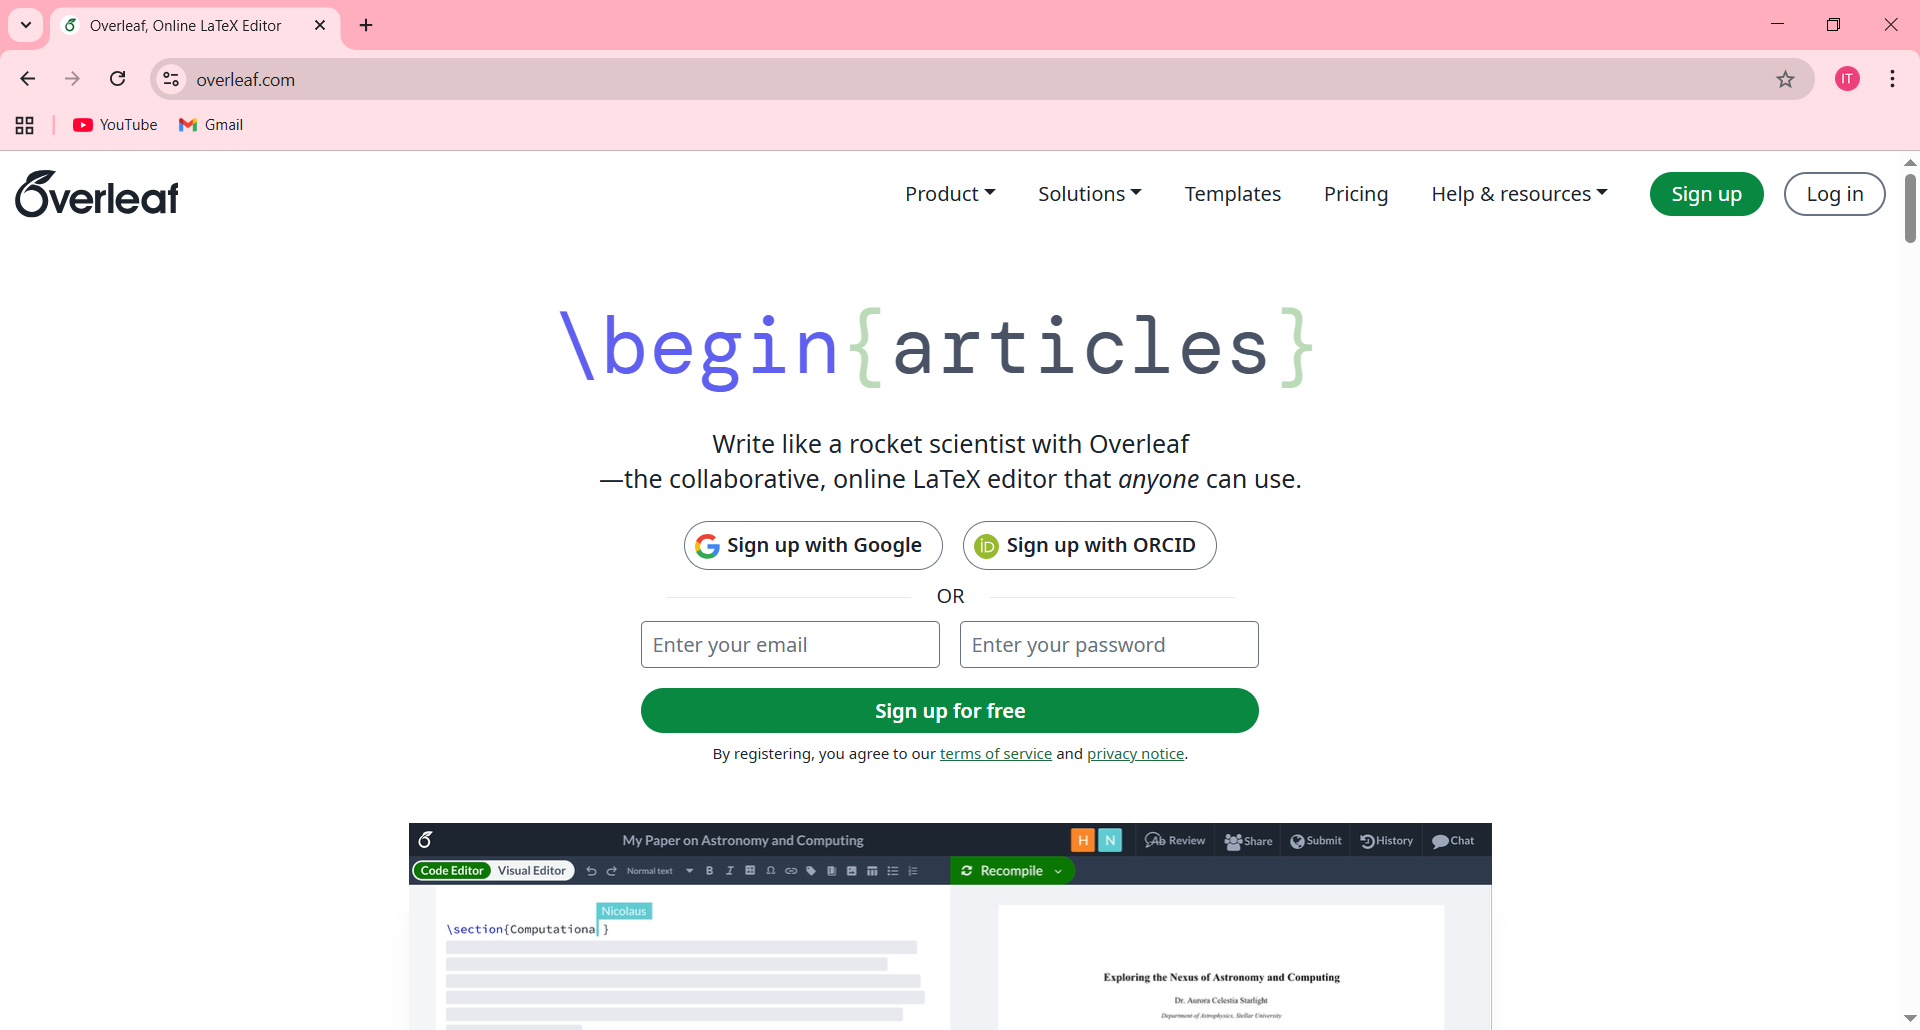
\includegraphics[width=0.8\textwidth]{Image/Overfeaf-1.png}
}
\caption{\fontSixTeen{หน้าแรกของเว็บไซต์ Overleaf}}
\label{figA:WebSiteOverleaf1}
\end{figure}

    \item ที่หน้าแรกดังภาพที่ \ref{figA:WebSiteOverleaf1} ในกรณีที่ยังไม่ได้เป็นสมาชิกให้คลิกที่ \enquote{Sign up} ก็จะพบกับหน้าจอดังภาพที่ \ref{figA:WebSiteOverleaf2}

\begin{figure}[htbp]
\centering
\adjustbox{frame, width=0.8\textwidth}{
    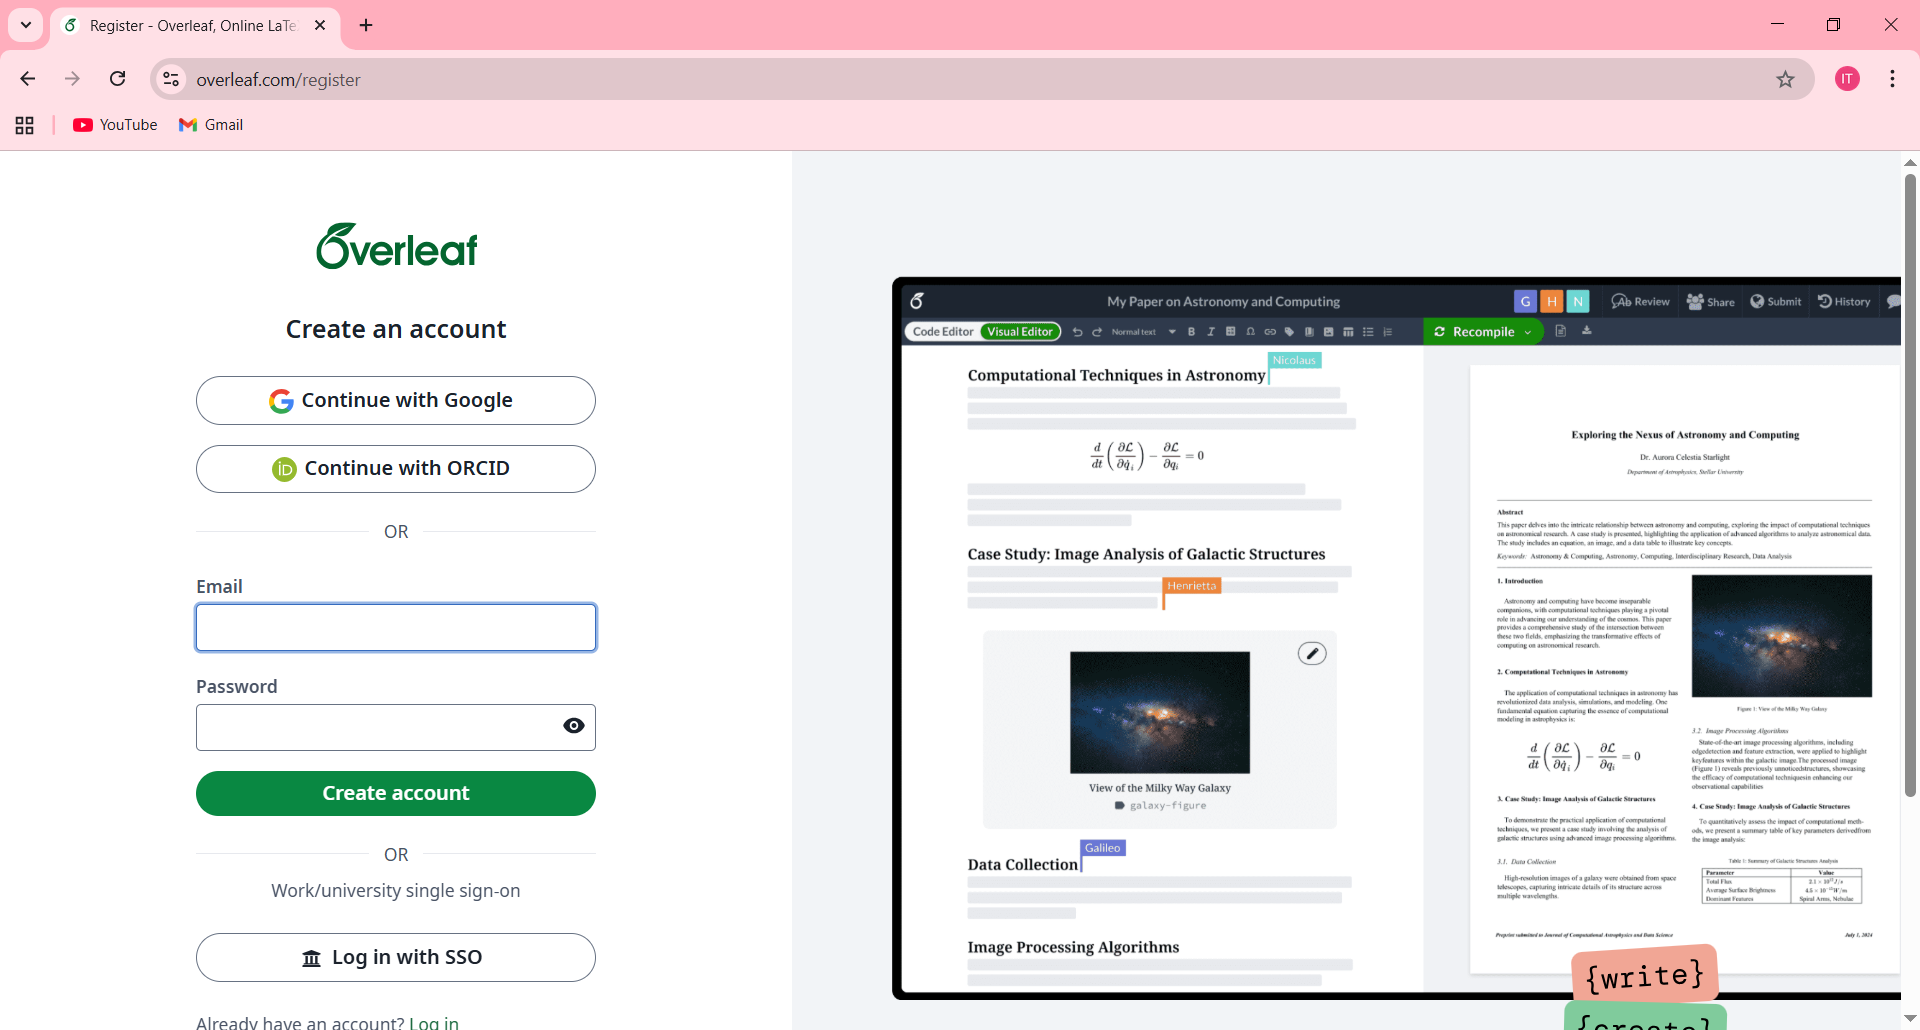
\includegraphics[width=0.8\textwidth]{Image/Overfeaf-2.png}
}
\caption{\fontSixTeen{หน้า Sign up ของเว็บไซต์ Overleaf}}
\label{figA:WebSiteOverleaf2}
\end{figure}

    \item ผู้ใช้งานสามารถเลือกสมัครสมาชิกได้หลายวิธี เช่น
    \begin{mycustomenum2}
        \item สมัครด้วยอีเมล โดยกรอกชื่อ อีเมล และรหัสผ่านที่ต้องการ
        \item สมัครด้วย Google mail ซึ่งเป็นวิธีที่ง่ายและรวดเร็ว 
        \begin{mycustomenum2}
            \item หลังจากคลิกที่ \enquote{Continue with Google} แสดงได้ดังภาพที่ \ref{figA:WebSiteOverleaf3}

\begin{figure}[htbp]
\centering
\adjustbox{frame, width=0.8\textwidth}{
    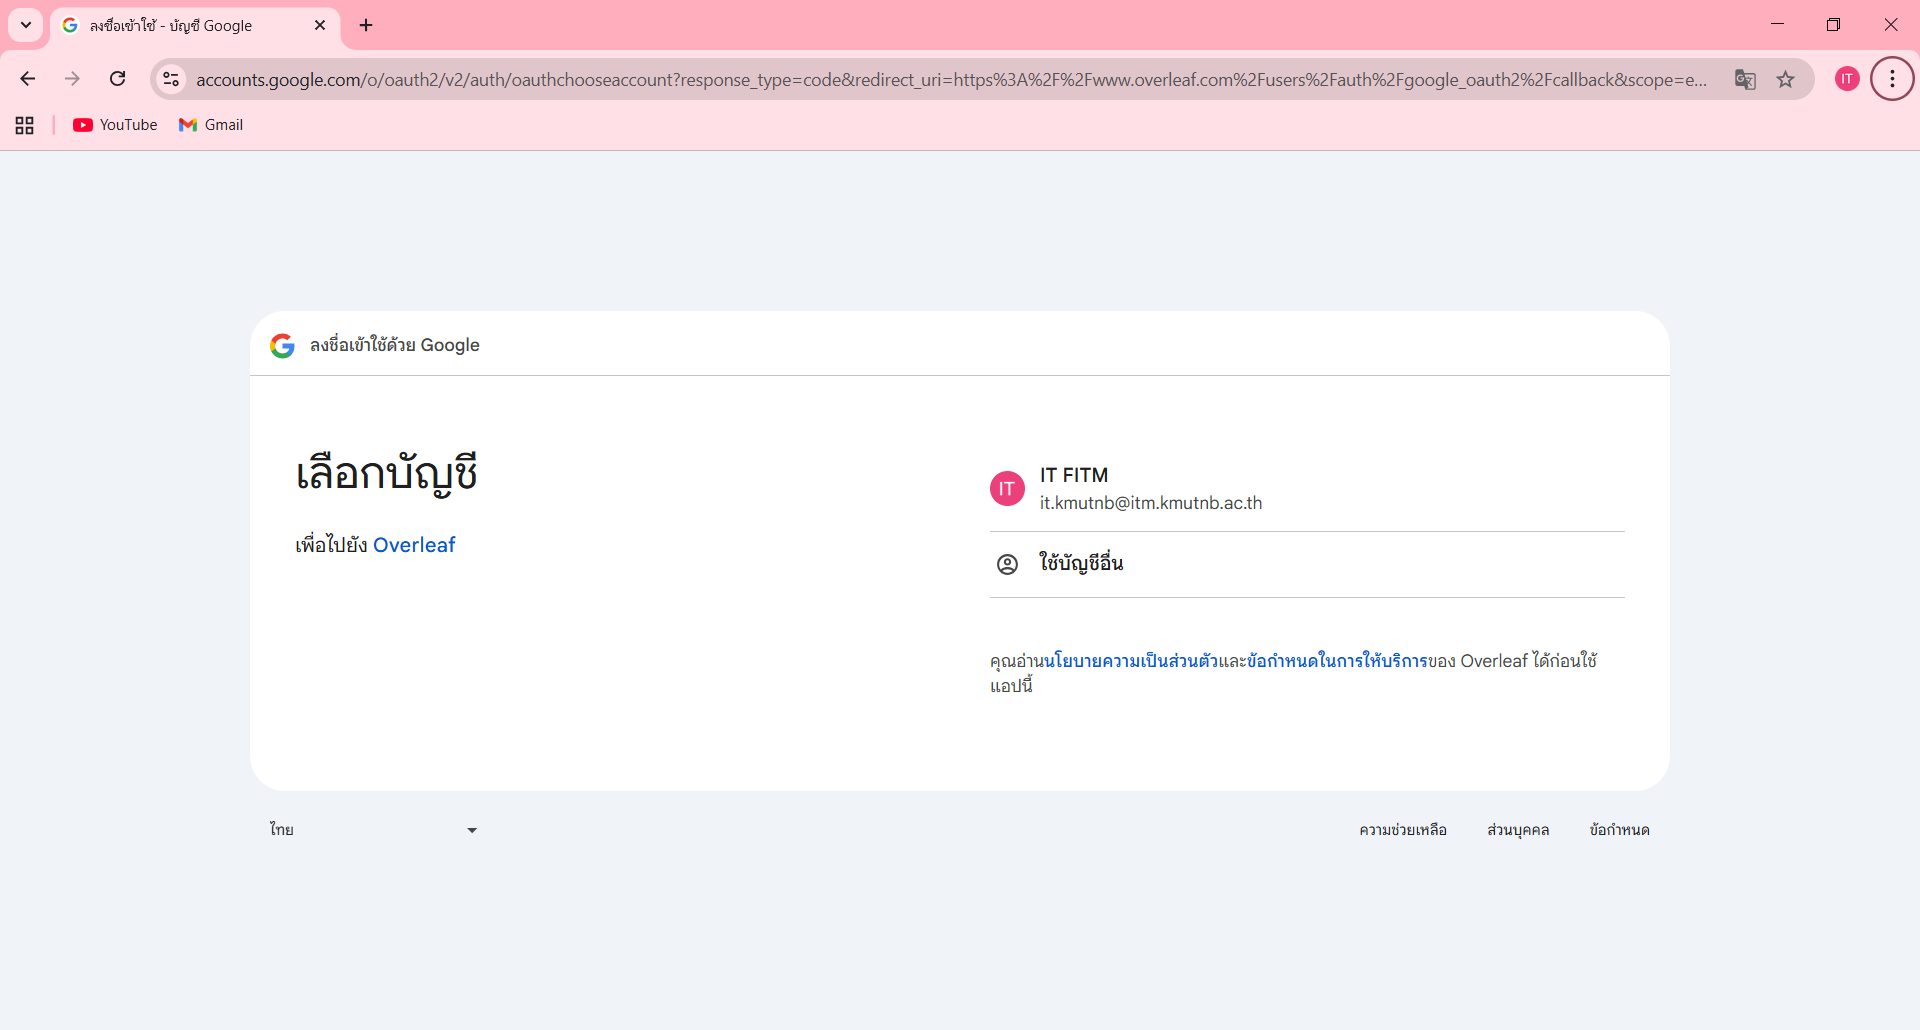
\includegraphics[width=0.8\textwidth]{Image/Overfeaf-3.png}
}
\caption{\fontSixTeen{หน้าเลือกบัญชี Google สำหรับสมัครสมาชิก}}
\label{figA:WebSiteOverleaf3}
\end{figure}

            \item คลิกเลือกบัญชีที่ต้องการเชื่อมต่อ แสดงดังภาพที่ \ref{figA:WebSiteOverleaf4}

\begin{figure}[htbp]
\centering
\adjustbox{frame, width=0.8\textwidth}{
    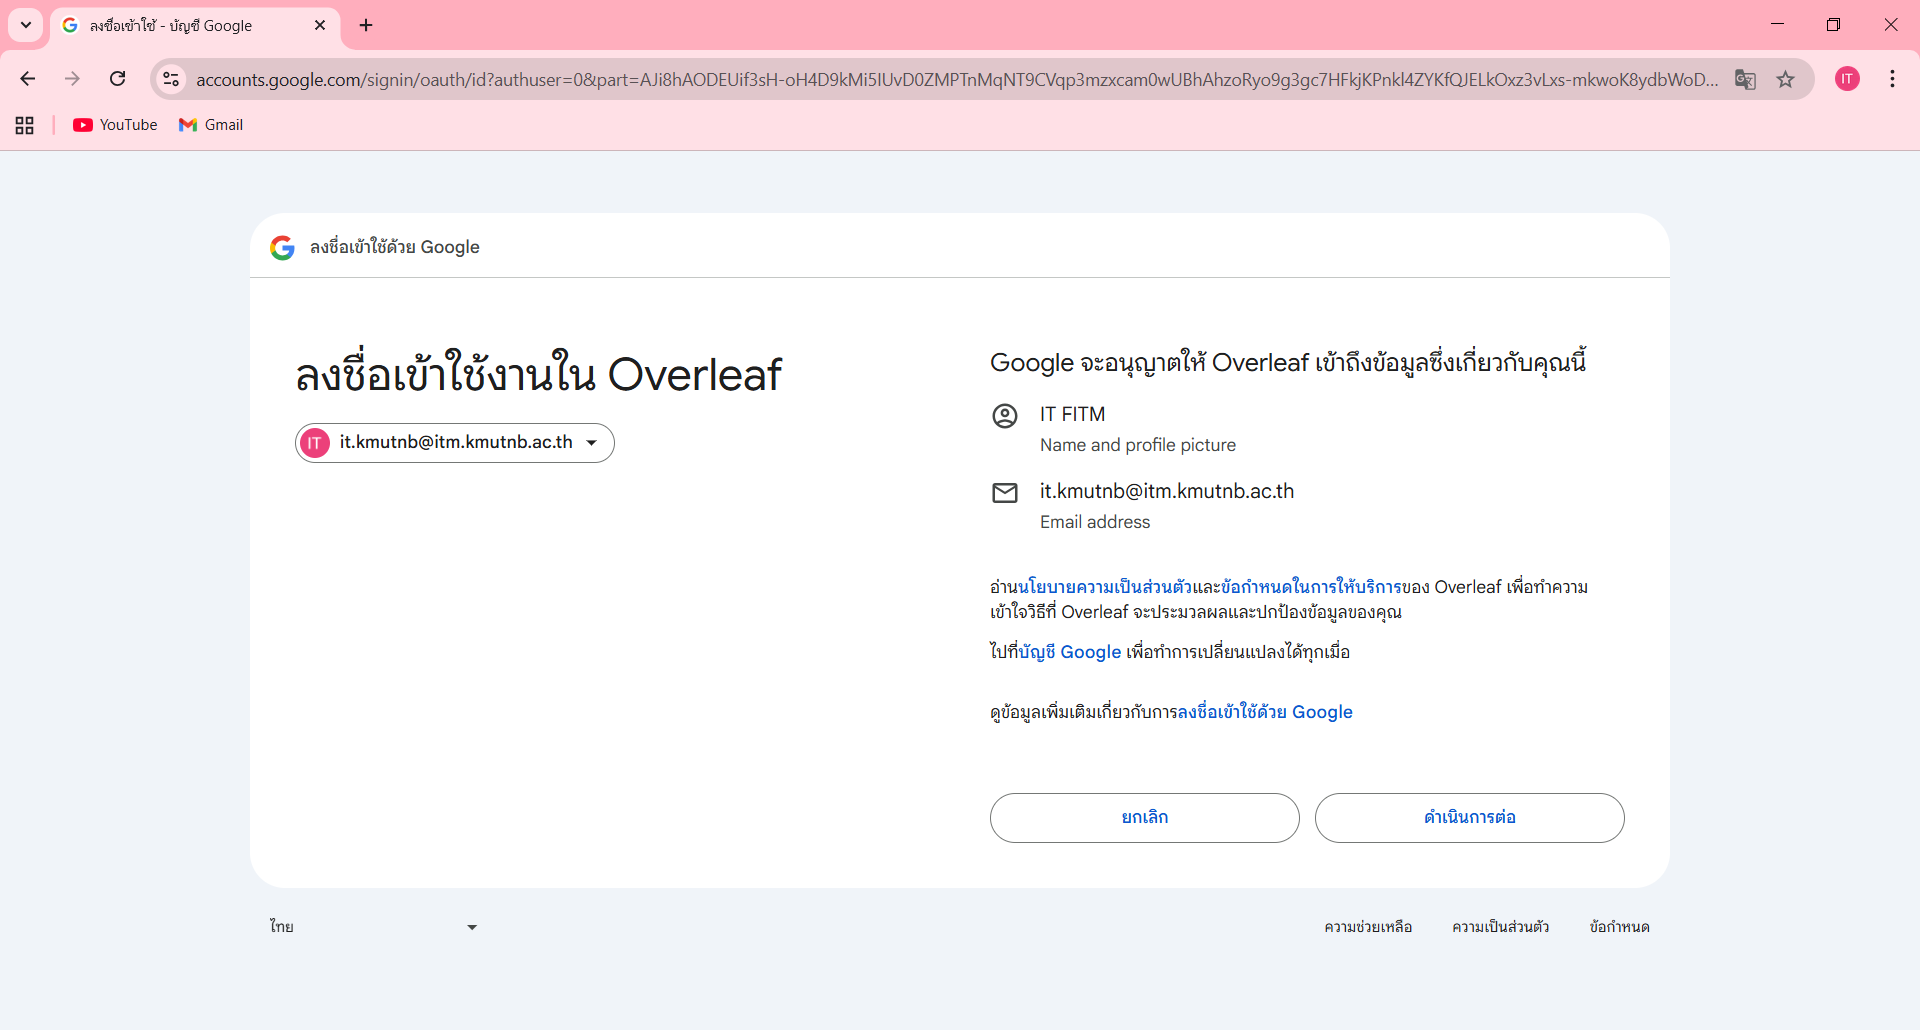
\includegraphics[width=0.8\textwidth]{Image/Overfeaf-4.png}
}
\caption{\fontSixTeen{หน้ายืนยันให้ Overleaf เข้าถึงข้อมูล}}
\label{figA:WebSiteOverleaf4}
\end{figure}

            \item คลิกที่ \enquote{ดำเนินการต่อ} แสดงดังภาพที่ \ref{figA:WebSiteOverleaf5} และให้คลิกที่ คำว่า \enquote{skip}

\begin{figure}[htbp]
\centering
\adjustbox{frame, width=0.8\textwidth}{
    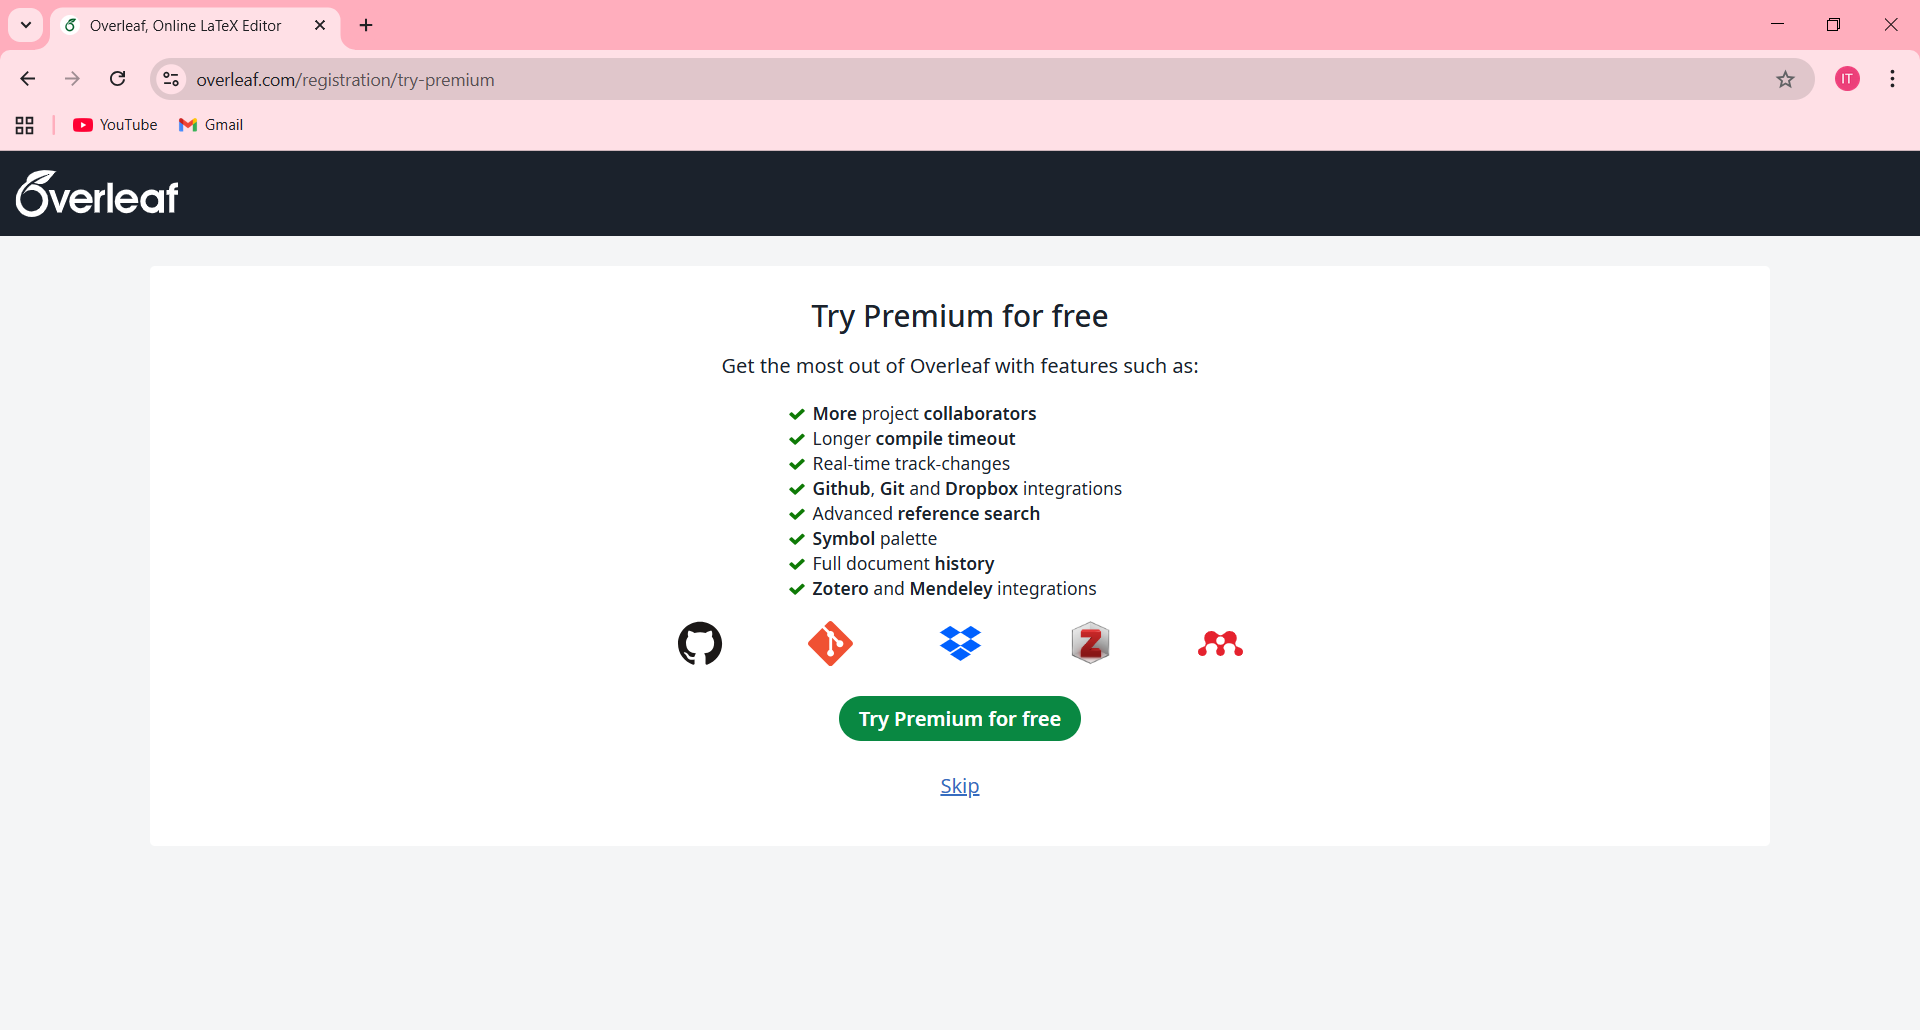
\includegraphics[width=0.8\textwidth]{Image/Overfeaf-5.png}
}
\caption{\fontSixTeen{หน้าเว็บไซต์ Overleaf หลังลงทะเบียน}}
\label{figA:WebSiteOverleaf5}
\end{figure}

            \item ตรวจสอบชื่อและนามสกุลว่าถูกต้องไหม ถ้าชื่อกับนามสกุลถูกต้อง ให้คลิกที่ \enquote{Continue} แสดงดังภาพที่ \ref{figA:WebSiteOverleaf6} \vspace{0.5em}

\begin{figure}[htbp]
\centering
\adjustbox{frame, width=0.8\textwidth}{
    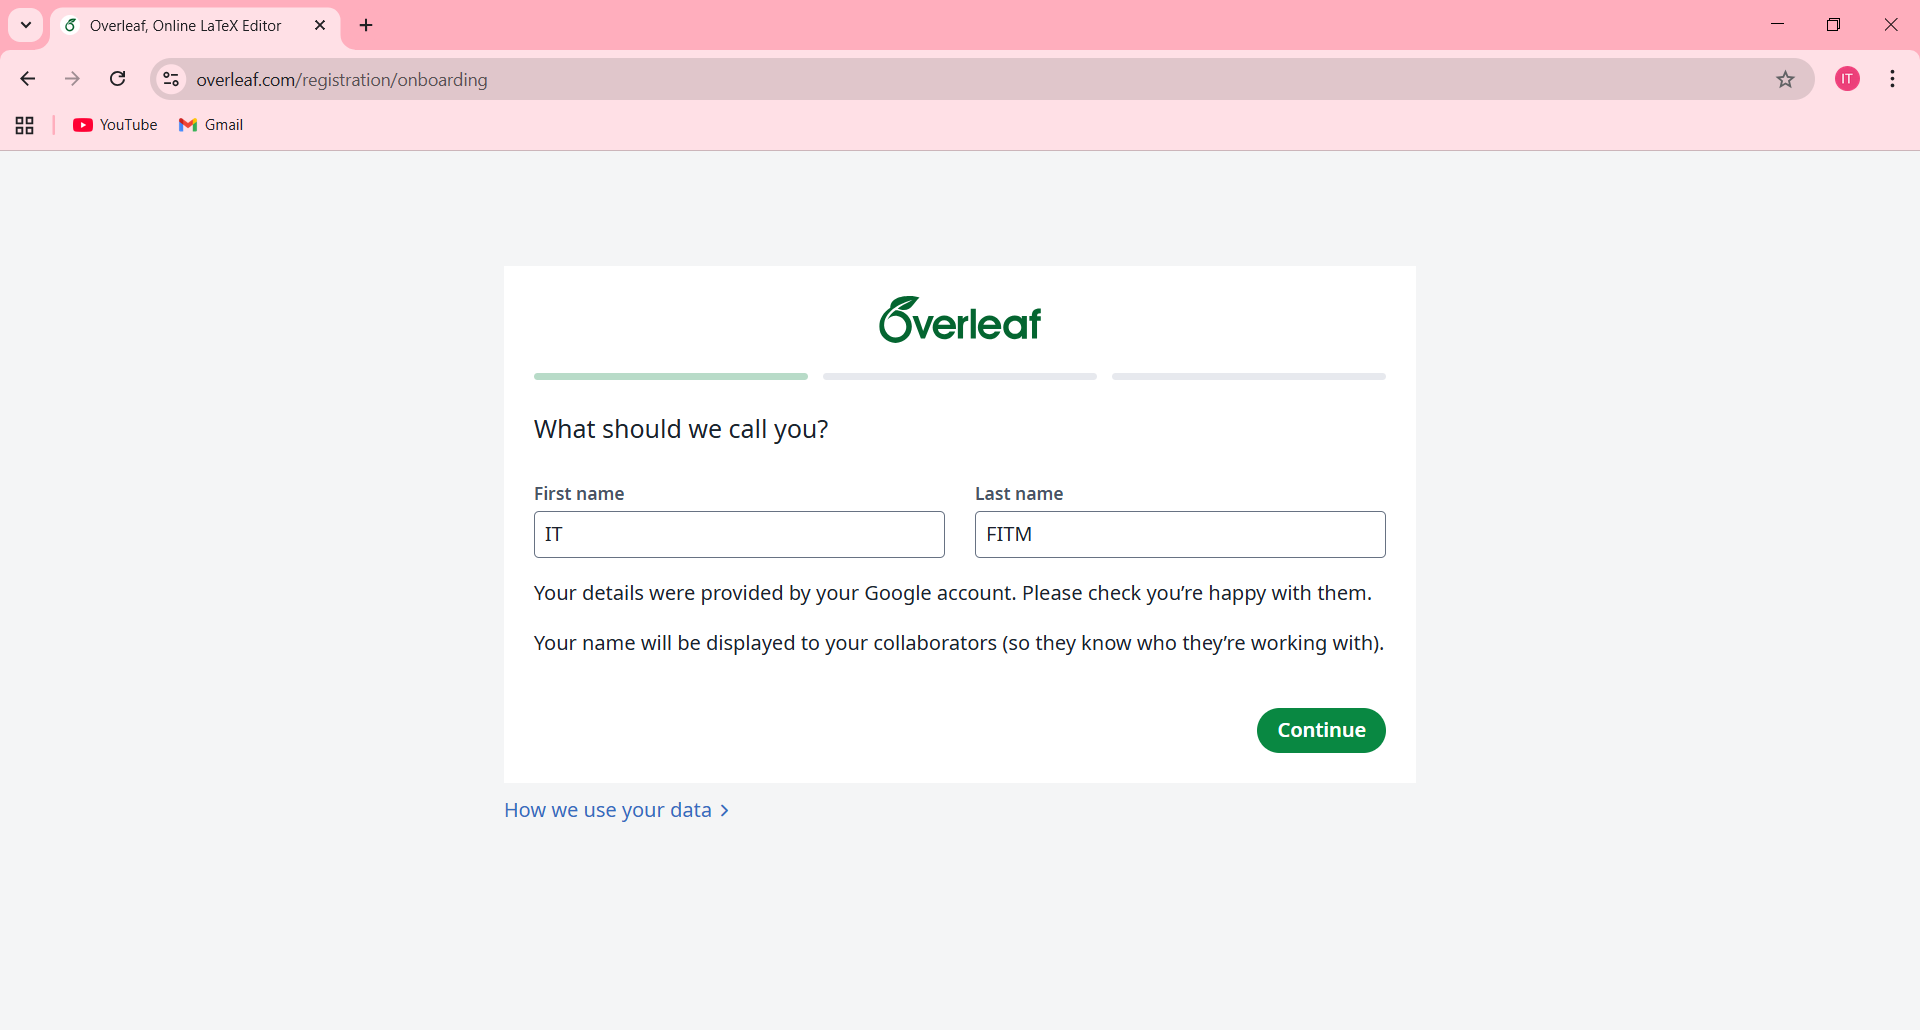
\includegraphics[width=0.8\textwidth]{Image/Overfeaf-6.png}
}
\caption{\fontSixTeen{หน้าตรวจสอบข้อมูลส่วนตัว}}
\label{figA:WebSiteOverleaf6}
\end{figure}

            \item จากนั้นก็ตอบคำถามทั่วไป แล้วคลิกที่ \enquote{Continue} และในหน้าสุดท้ายคลิกที่ \enquote{Go to Overleaf} ก็เป็นอันเสร็จสิ้น แสดงได้ดังภาพที่ \ref{figA:WebSiteOverleaf7} 

\begin{figure}[htbp]
\centering
\adjustbox{frame, width=0.8\textwidth}{
    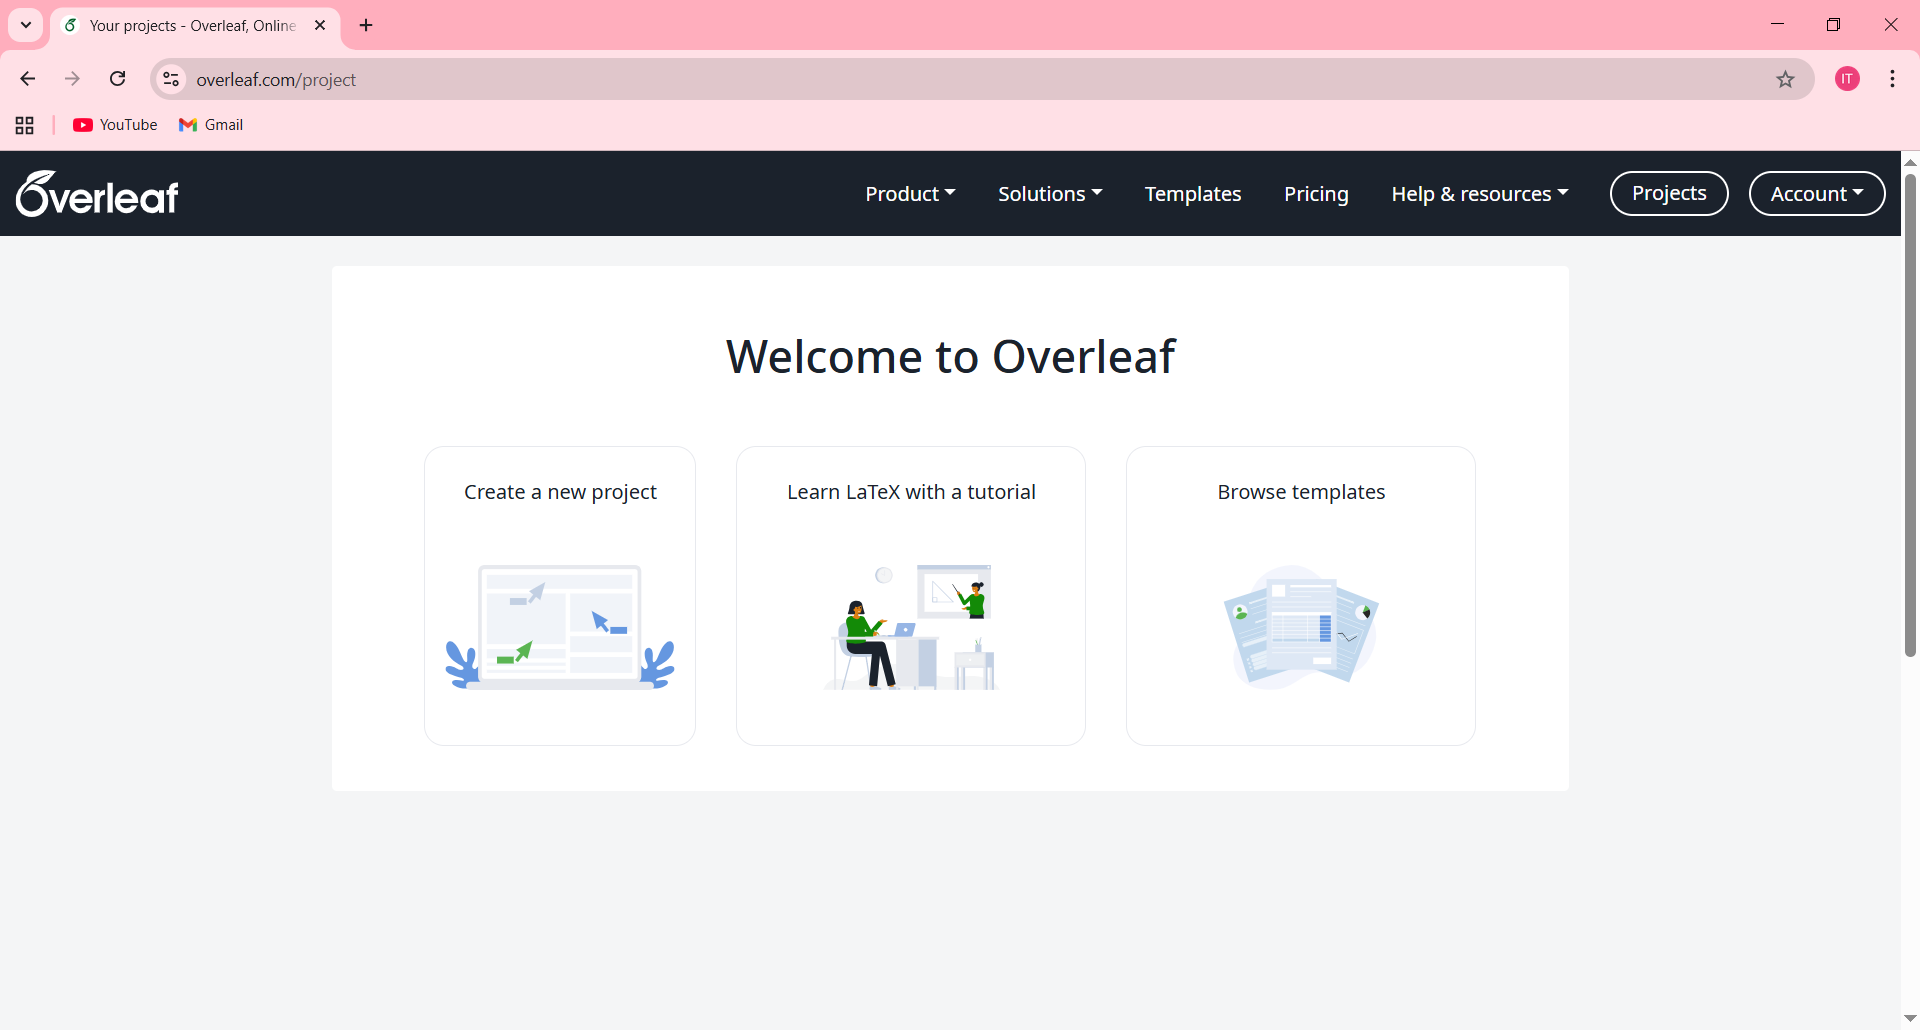
\includegraphics[width=0.8\textwidth]{Image/Overfeaf-7.png}
}
\caption{\fontSixTeen{หน้าแรกหลังจากลงทะเบียนเว็บไซต์ Overleaf สำเร็จแล้ว}}
\label{figA:WebSiteOverleaf7}
\end{figure}
                
        \end{mycustomenum2}   
    \end{mycustomenum2}   
    \item ที่หน้าแรกดังภาพที่ \ref{figA:WebSiteOverleaf1} ในกรณีที่เป็นสมาชิกให้คลิกที่ \enquote{Log in} และเลือก \enquote{Log in with Google} ก็จะพบกับหน้าจอดังภาพที่ \ref{figA:WebSiteOverleaf7}
    
    \item จากภาพที่ \ref{figA:WebSiteOverleaf7} ให้คลิกที่ \enquote{Create a new project} และเลือก \enquote{Upload project} แสดงได้ดังภาพที่ \ref{figA:WebSiteOverleaf8}

\begin{figure}[htbp]
\centering
\adjustbox{frame, width=0.8\textwidth}{
    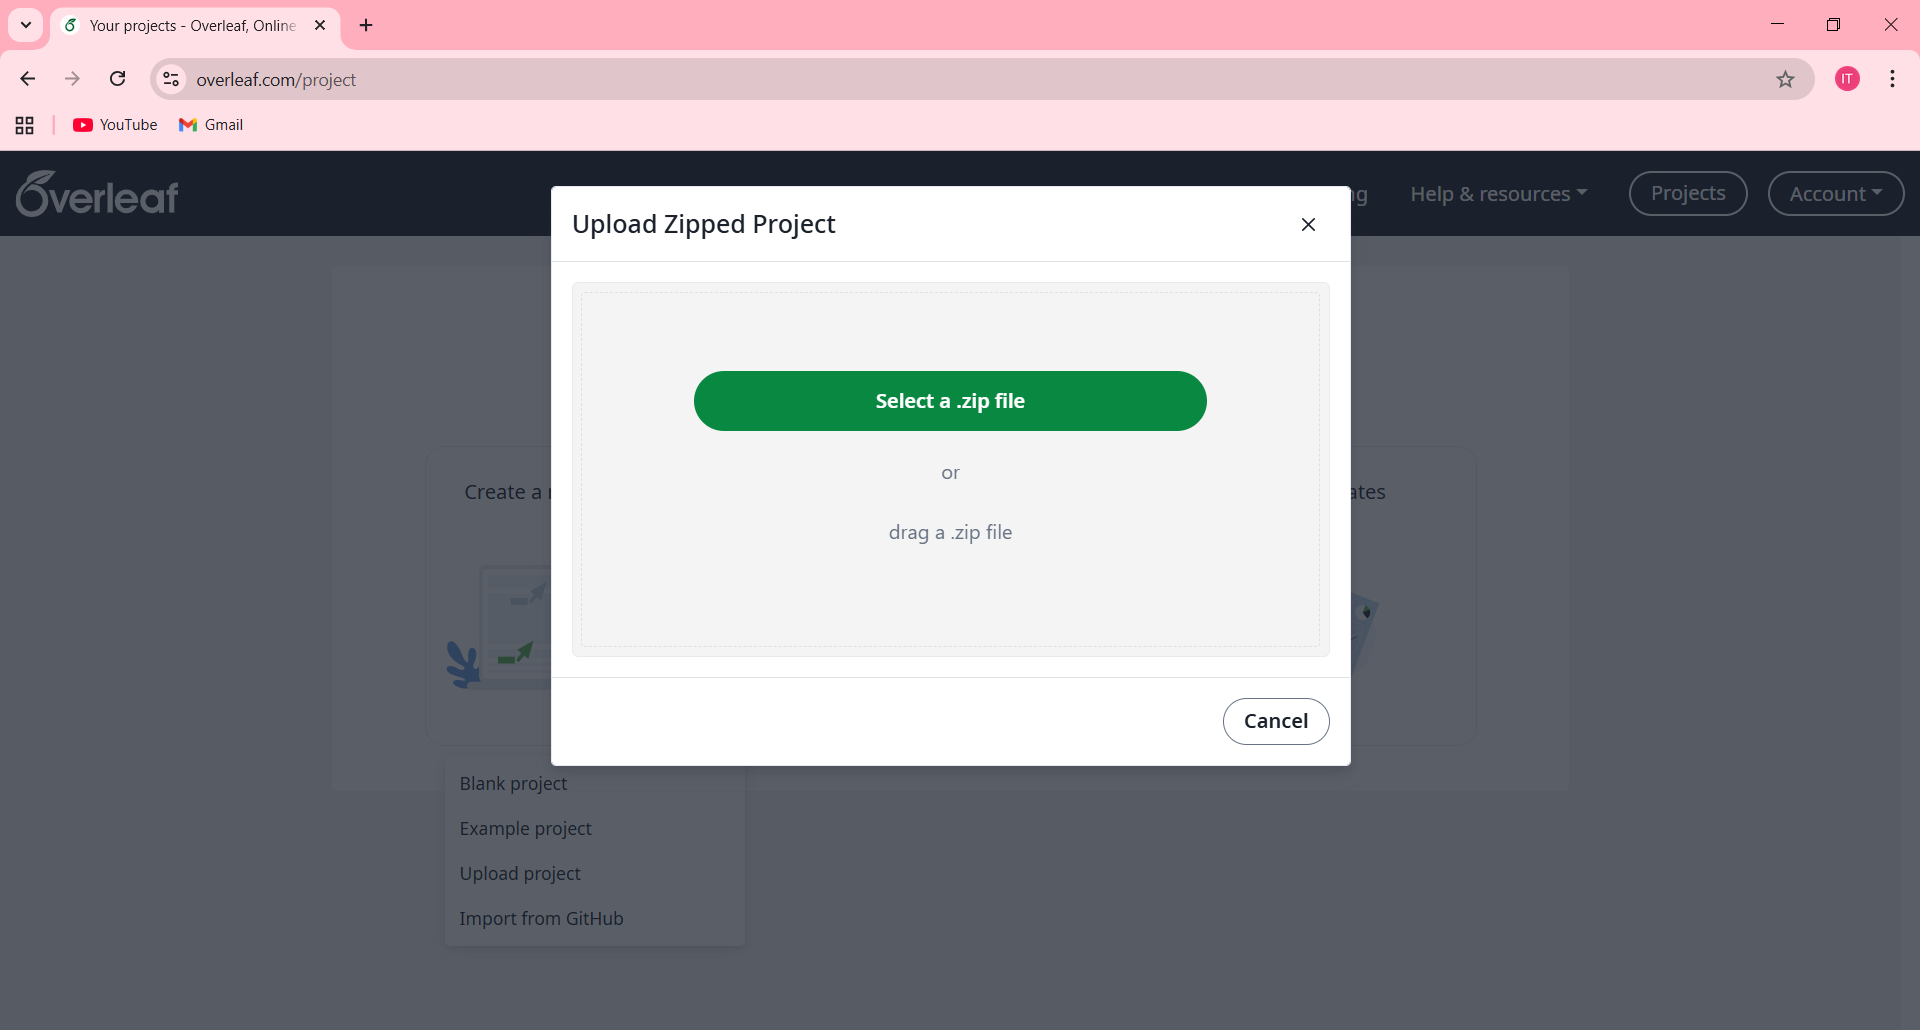
\includegraphics[width=0.8\textwidth]{Image/Overfeaf-8.png}
}
\caption{\fontSixTeen{หน้า Upload a .zip file}}
\label{figA:WebSiteOverleaf8}
\end{figure}

    \item เมื่อคลิกที่ \enquote{Upload a .zip file} และเลือกไฟล์ .zip ที่ upload ได้แล้ว ก็จะแสดงได้ดังภาพที่ \ref{figA:WebSiteOverleaf9}

\begin{figure}[htbp]
\centering
\adjustbox{frame, width=0.8\textwidth}{
    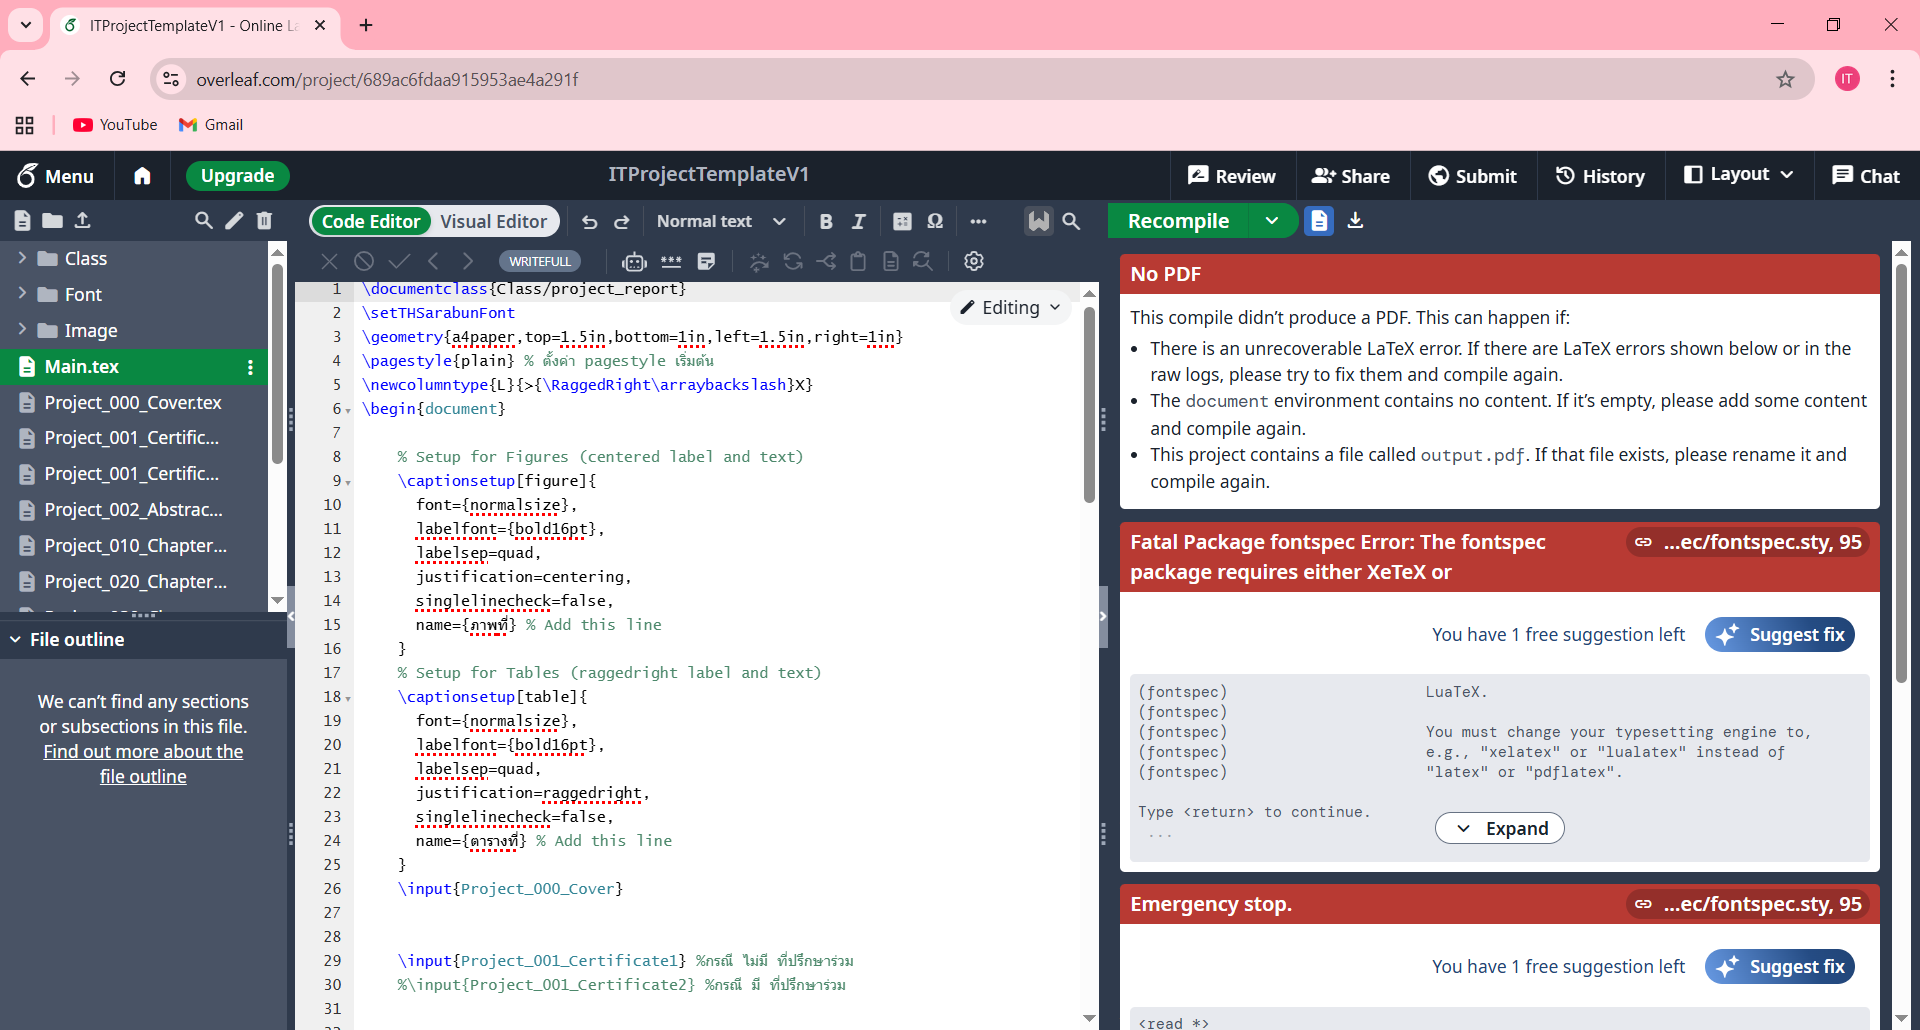
\includegraphics[width=0.8\textwidth]{Image/Overfeaf-9.png}
}
\caption{\fontSixTeen{หน้าสำหรับการแก้ไขเนื้อหาใน Overleaf}}
\label{figA:WebSiteOverleaf9}
\end{figure}

    \item จากภาพที่ \ref{figA:WebSiteOverleaf9} ให้คลิกที่ \enquote{Menu} ที่อยู่มุมซ้ายบน และที่ Compiler ให้เปลี่ยนเป็น \enquote{XeLaTex} และ Spell check ให้เป็น \enquote{Thai} ดังภาพที่ \ref{figA:WebSiteOverleaf10} 

\begin{figure}[htbp]
\centering
\adjustbox{frame, width=0.8\textwidth}{
    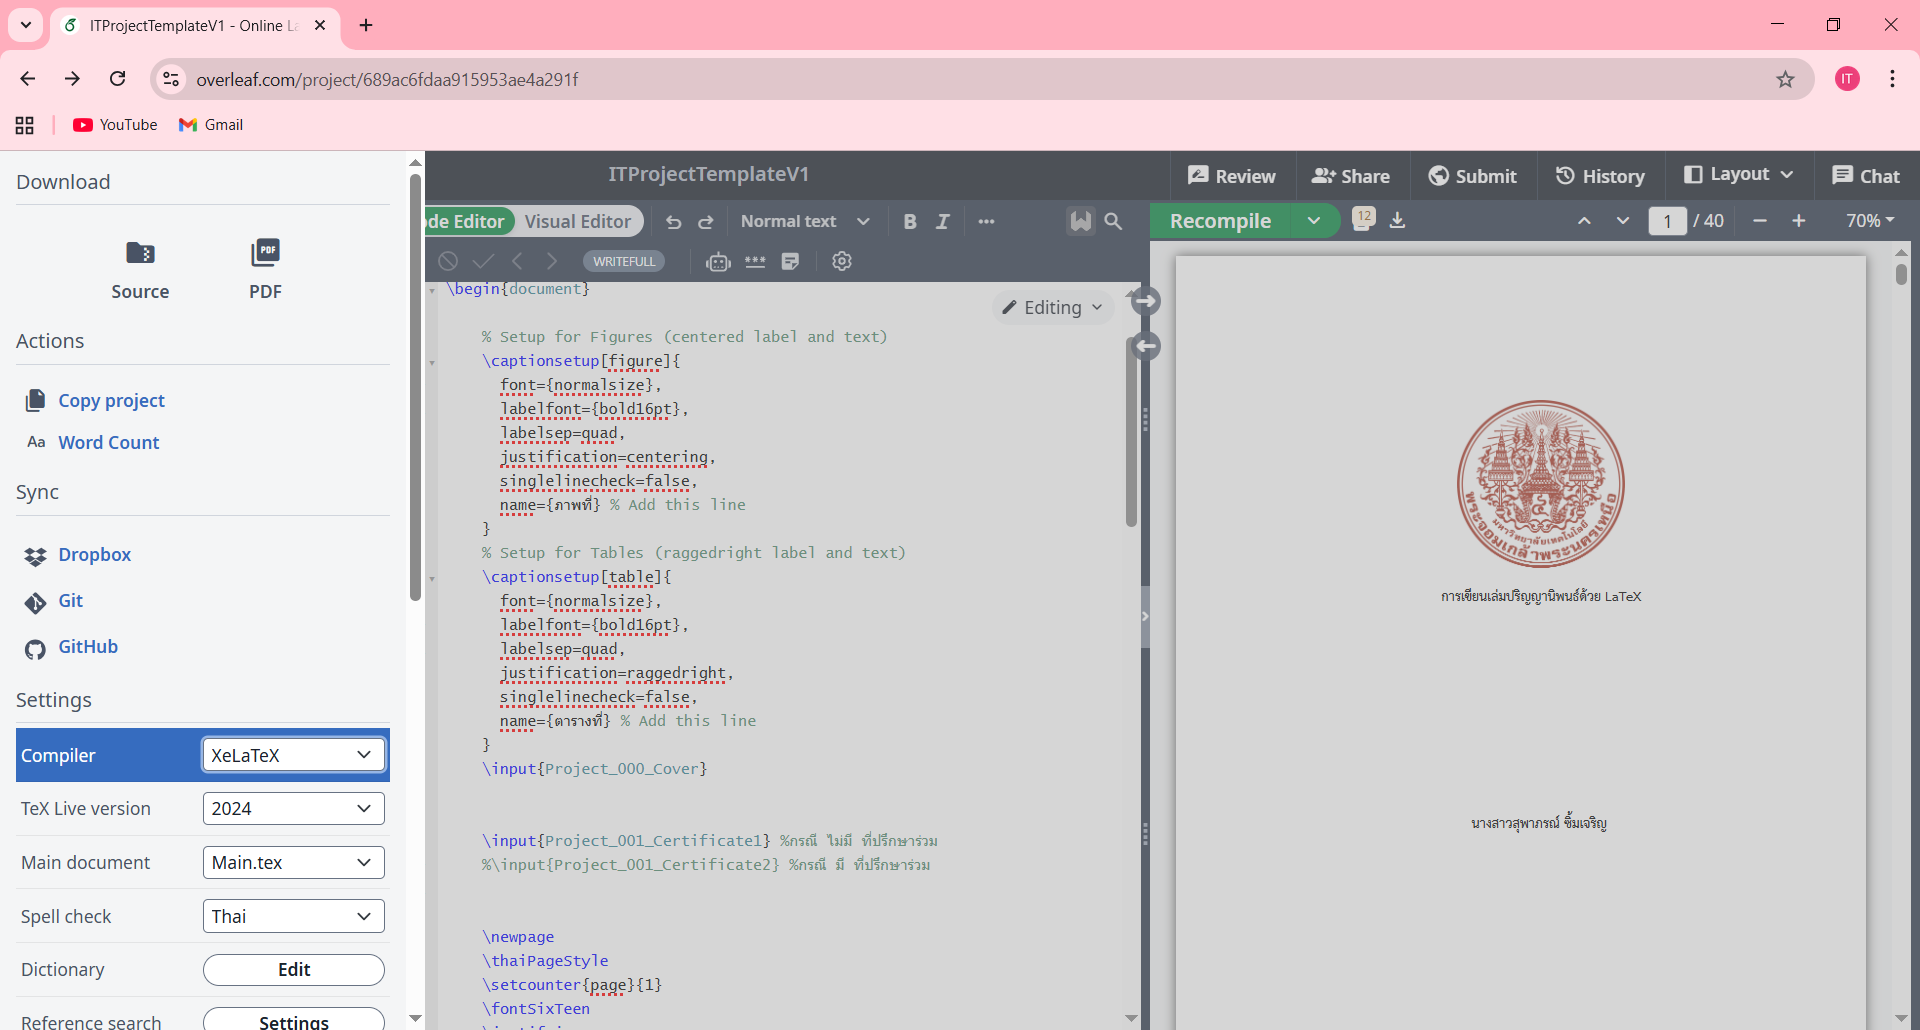
\includegraphics[width=0.8\textwidth]{Image/Overfeaf-10.png}
}
\caption{\fontSixTeen{หน้าสำหรับเปลี่ยน Compiler และ Spell check}}
\label{figA:WebSiteOverleaf10}
\end{figure}

    \item เมื่อคลิกที่ \enquote{Recompile} Error ก็จะหายไป แสดงได้ดังภาพที่  \ref{figA:WebSiteOverleaf11}

\begin{figure}[htbp]
\centering
\adjustbox{frame, width=0.8\textwidth}{
    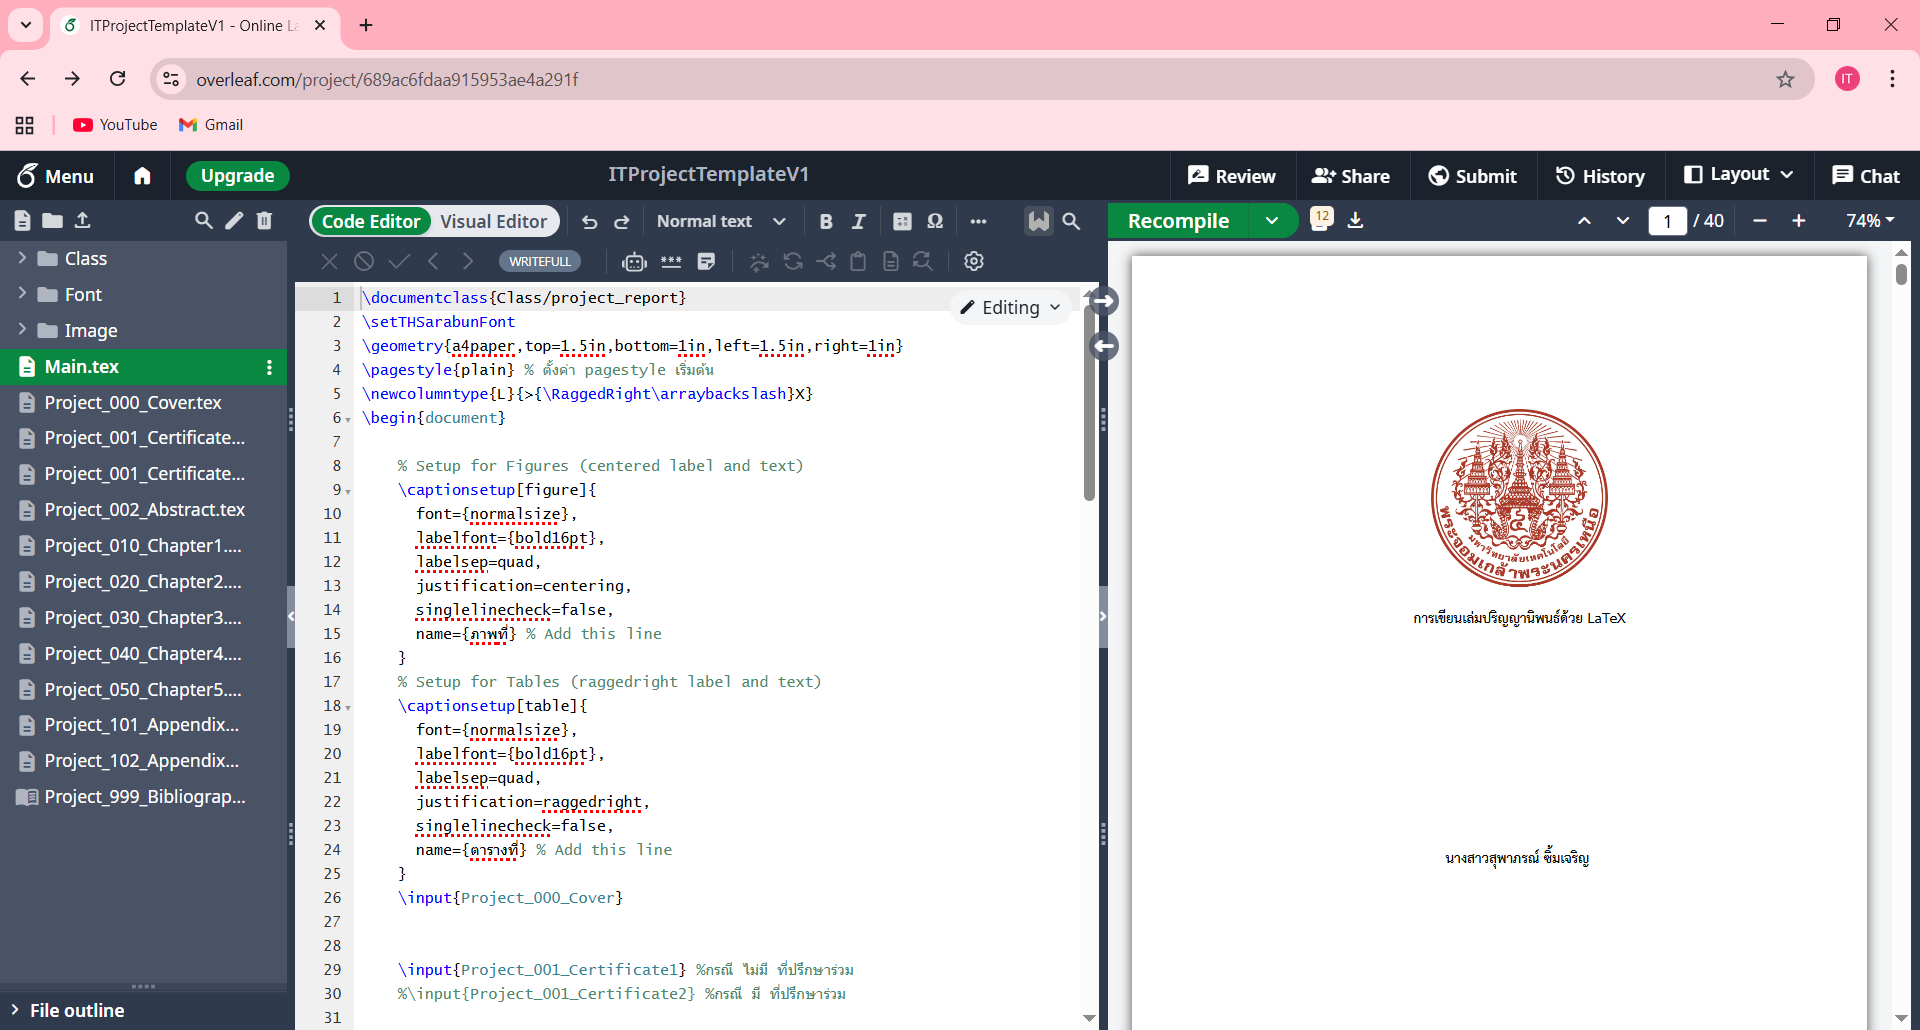
\includegraphics[width=0.8\textwidth]{Image/Overfeaf-11.png}
}
\caption{\fontSixTeen{หน้าหลังจากที่เปลี่ยน Compile เป็น "XeLaTex"}}
\label{figA:WebSiteOverleaf11}
\end{figure}

    \item เมื่อต้องการกลับหน้ารวม Project ให้คลิกที่ icon \enquote{รูปบ้าน} ที่มุมบนซ้าย ก็จะไปยังหน้า Home ที่รวมโปรเจ็คทั้งหมด แสดงได้ดังภาพที่ \ref{figA:WebSiteOverleaf12}

\begin{figure}[htbp]
\centering
\adjustbox{frame, width=0.8\textwidth}{
    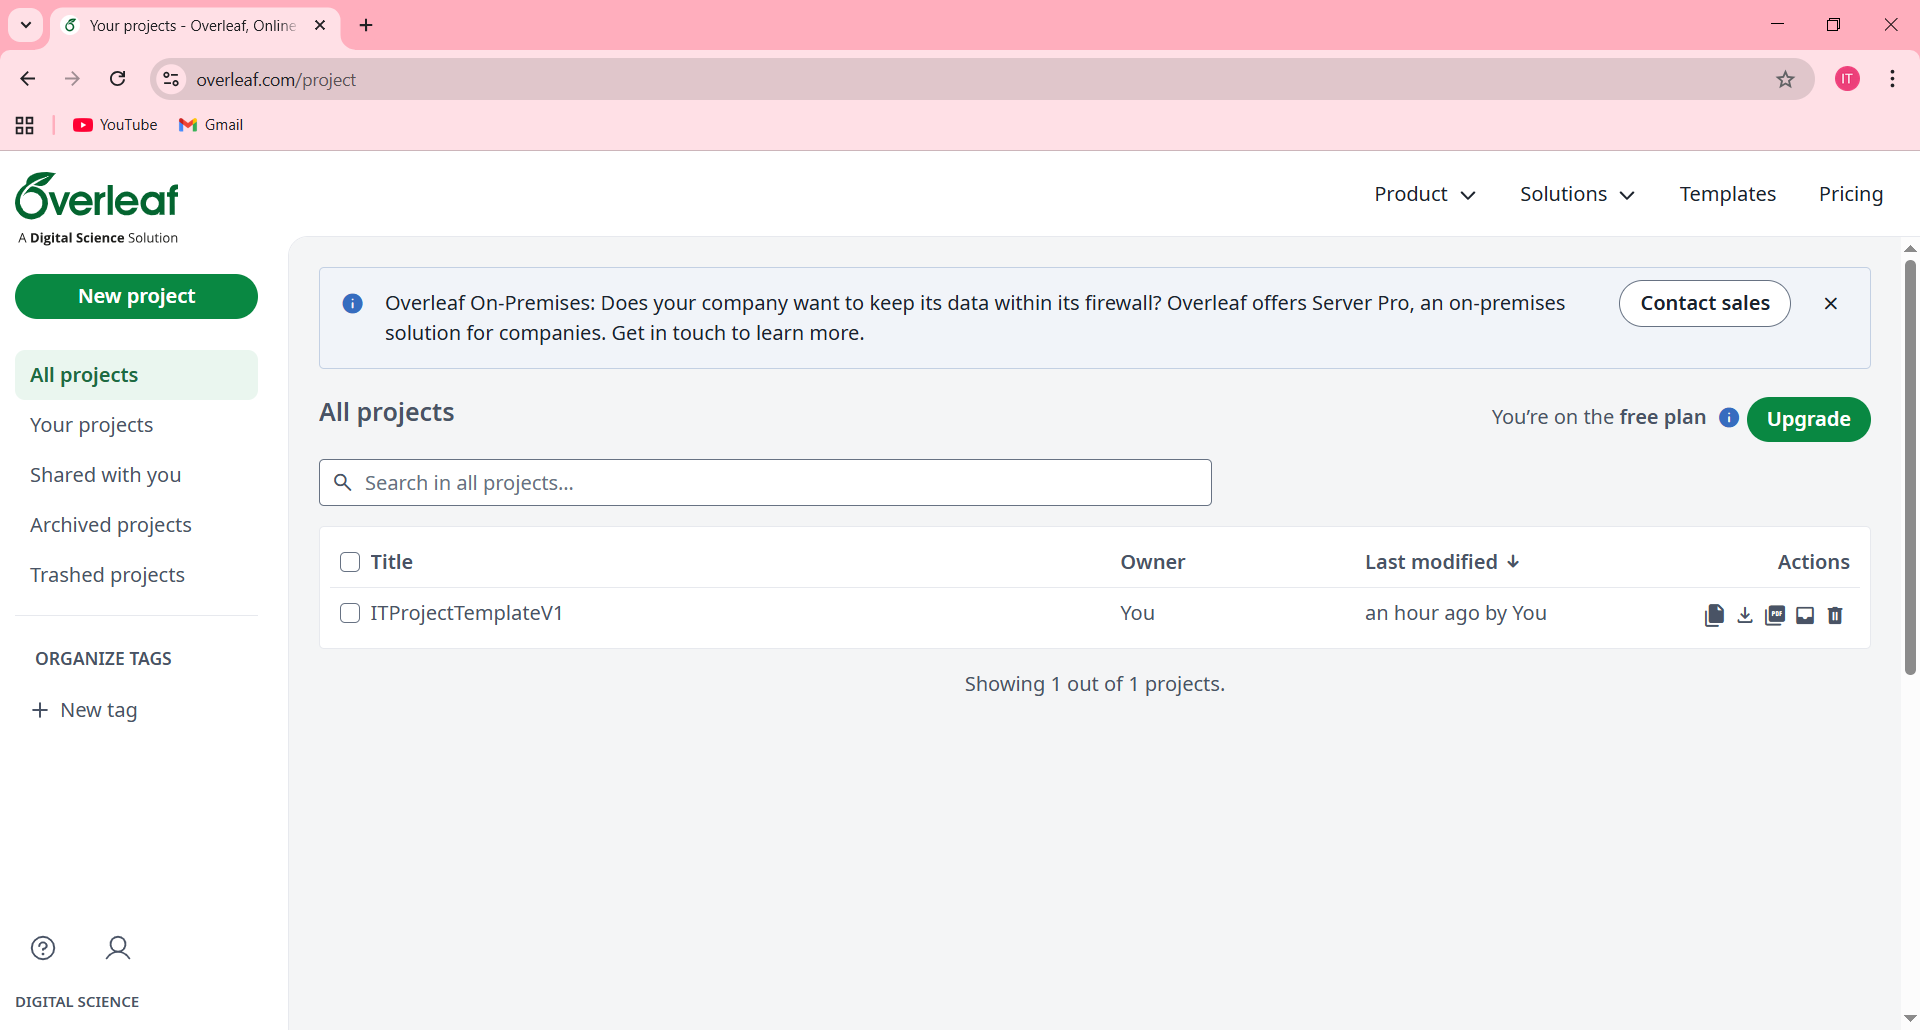
\includegraphics[width=0.8\textwidth]{Image/Overfeaf-12.png}
}
\caption{\fontSixTeen{หน้าสำหรับเปลี่ยน Compiler}}
\label{figA:WebSiteOverleaf12}
\end{figure}

\end{mycustomenum2}
